\label{sec:testing}
\section{Результаты тестирования программной разработки}


\begin{figure}[H]
    Пример с нулевыми векторами
    \vspace{0.3cm}
    

    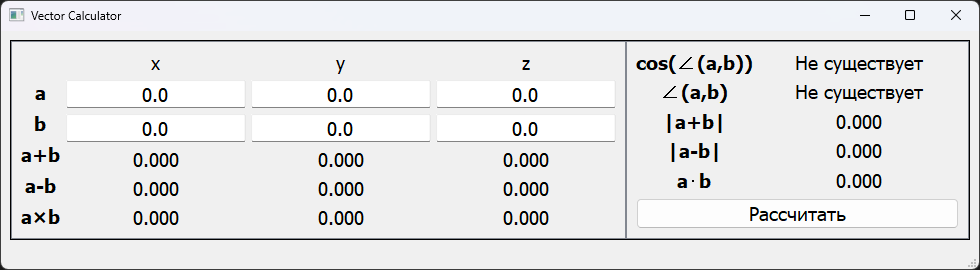
\includegraphics[width=\textwidth]{img//test1}
    \caption{}
\end{figure}

\begin{figure}[H]
    Пример с "египетским треугольником"
    \vspace{0.3cm}
    

    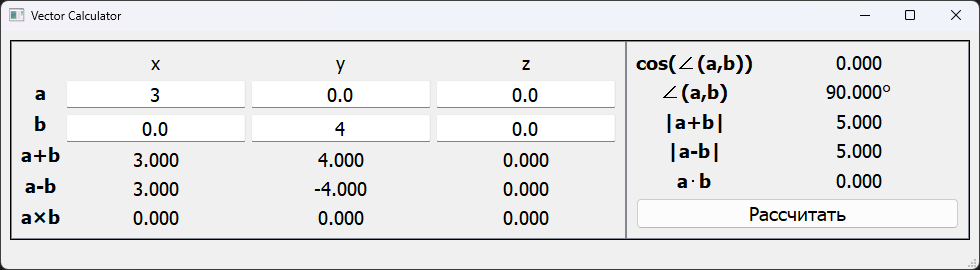
\includegraphics[width=\textwidth]{img//test2}
    \caption{}
\end{figure}

\begin{figure}[H]
    Пример с равнобедренным прямоугольным треугольником
    \vspace{0.3cm}
    

    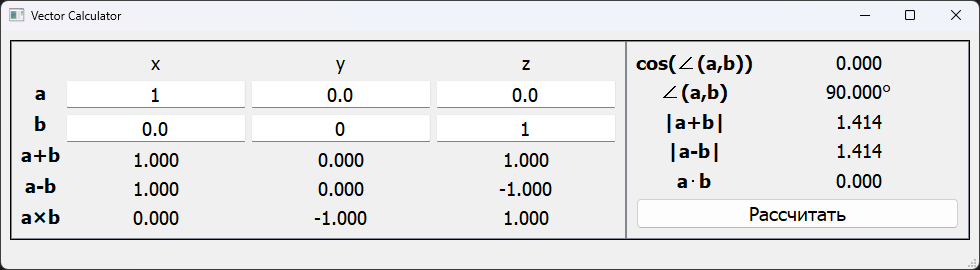
\includegraphics[width=\textwidth]{img//test3}
    \caption{}
\end{figure}

\begin{figure}[H]
    Пример с большими числами
    \vspace{0.3cm}
    

    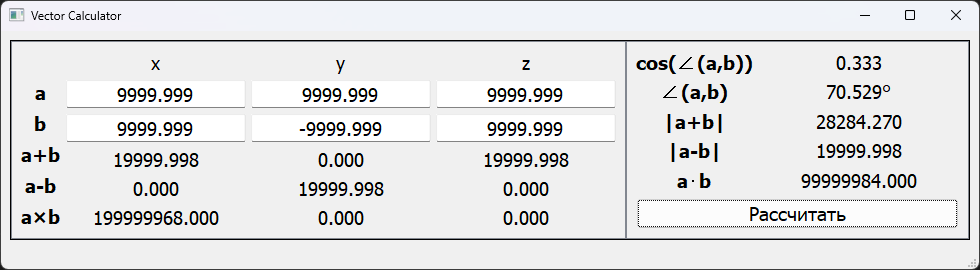
\includegraphics[width=\textwidth]{img//test4}
    \caption{}
\end{figure}